\documentclass{standalone}
\usepackage{tikz}
\usetikzlibrary{patterns, positioning}
\usepackage[sfdefault]{ClearSans} %% option 'sfdefault' activates Clear Sans as the default text font
\usepackage[T1]{fontenc}

\begin{document}
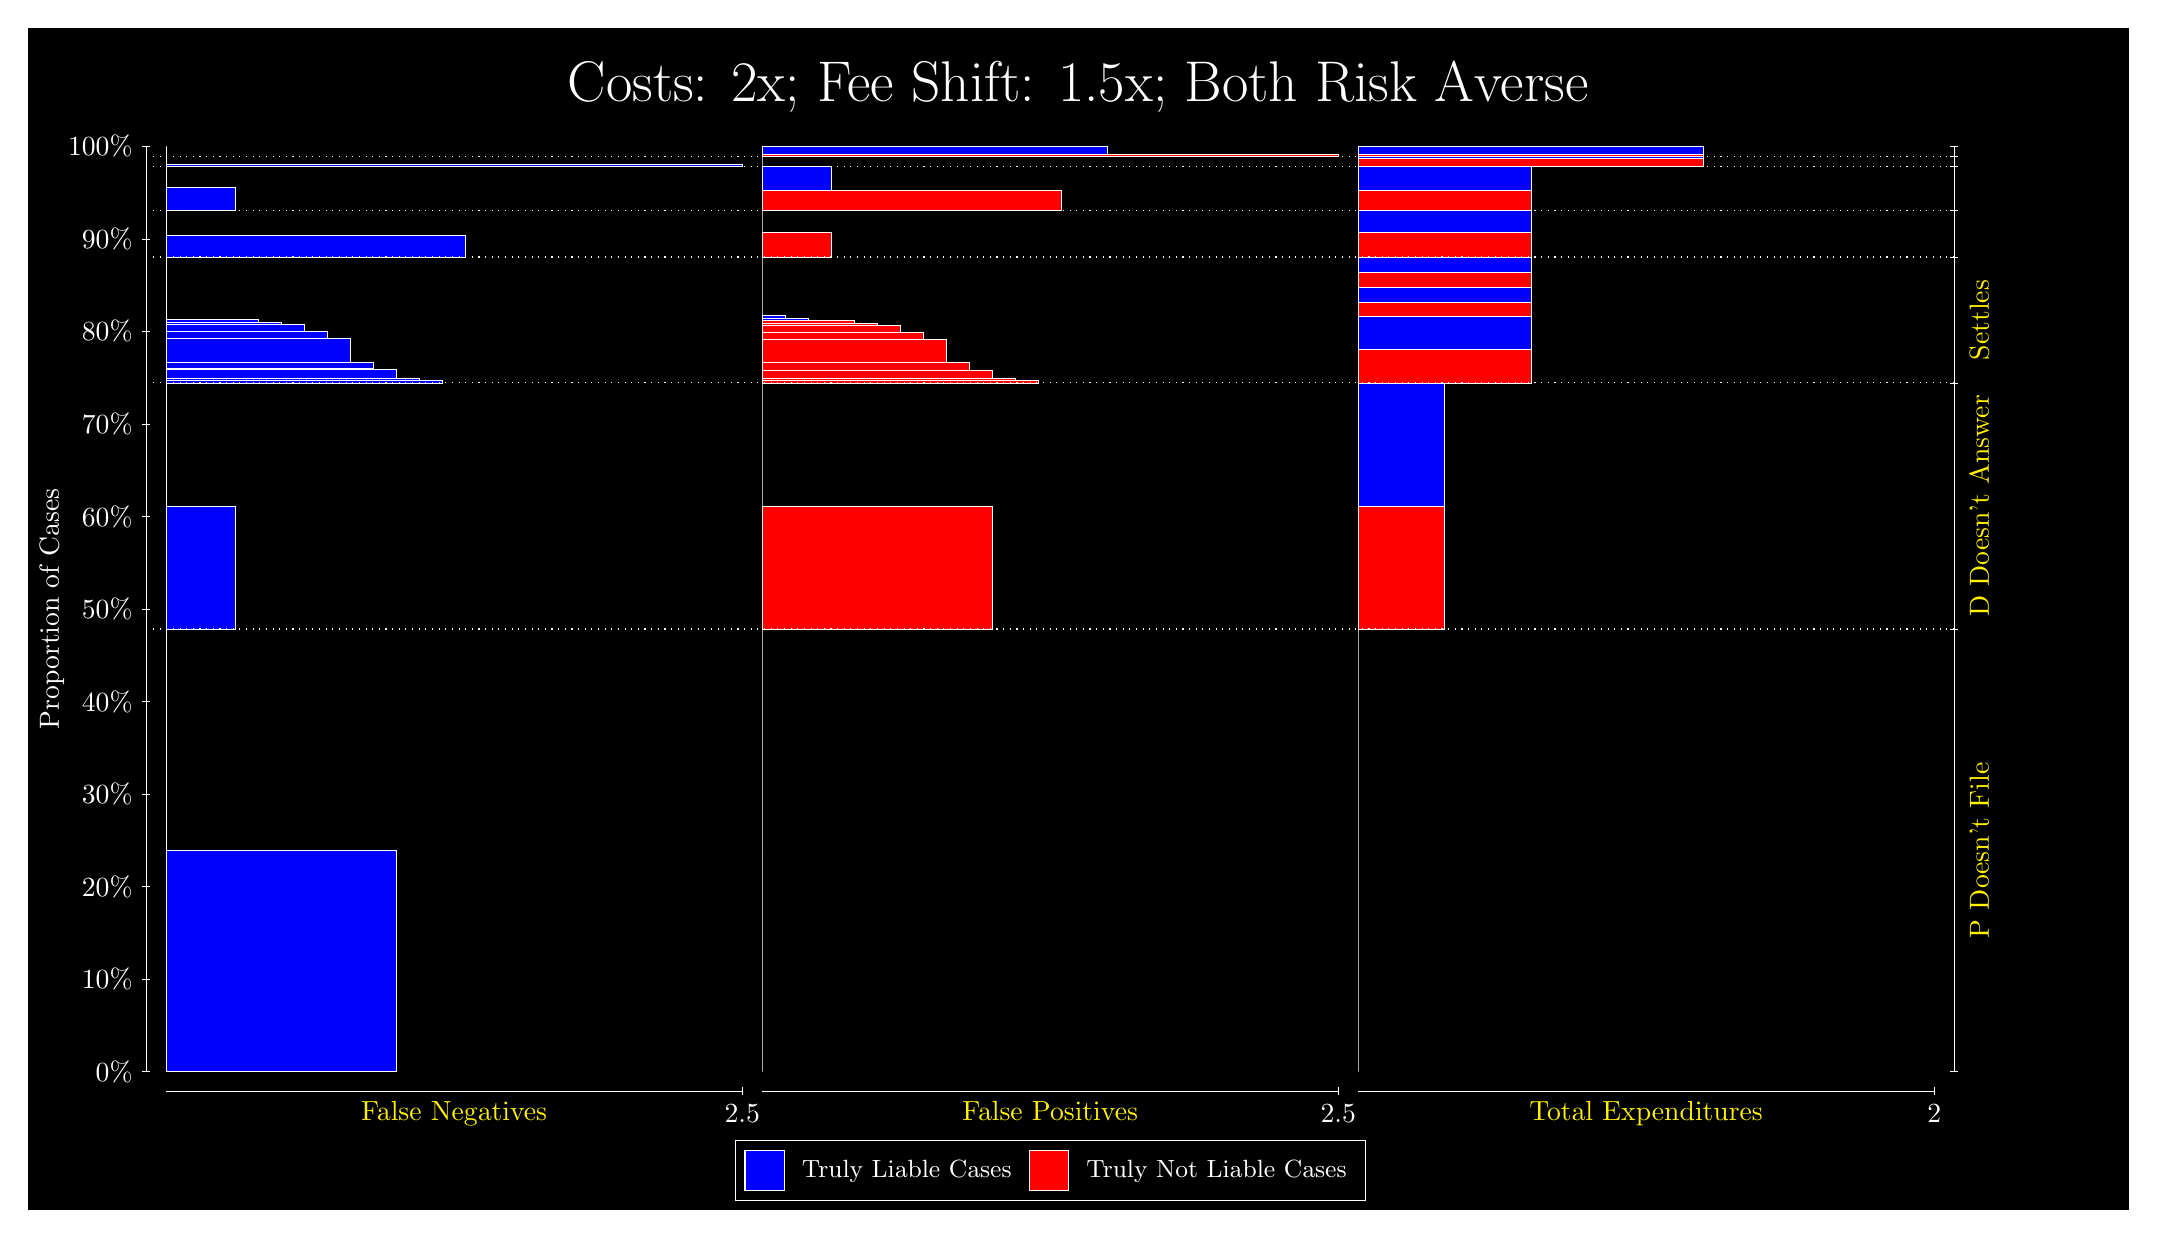
\begin{tikzpicture}
\draw[fill=black] (0,0) rectangle (26.667,15);
\draw[text=white] (0,13.5) rectangle (26.667,15) node[midway] {\huge Costs: 2x; Fee Shift: 1.5x; Both Risk Averse};
\draw[white, very thin] (1.5,1.75) -- (1.5,13.5);
\node[rotate=90, text=white, anchor=center] at (0.3, 7.625) {Proportion of Cases};
\draw[white, very thin] (1.45,1.75) -- (1.55,1.75);
\node[text=white, anchor=east] at (1.45, 1.75) {0\%};
\draw[white, very thin] (1.45,2.925) -- (1.55,2.925);
\node[text=white, anchor=east] at (1.45, 2.925) {10\%};
\draw[white, very thin] (1.45,4.1) -- (1.55,4.1);
\node[text=white, anchor=east] at (1.45, 4.1) {20\%};
\draw[white, very thin] (1.45,5.275) -- (1.55,5.275);
\node[text=white, anchor=east] at (1.45, 5.275) {30\%};
\draw[white, very thin] (1.45,6.45) -- (1.55,6.45);
\node[text=white, anchor=east] at (1.45, 6.45) {40\%};
\draw[white, very thin] (1.45,7.625) -- (1.55,7.625);
\node[text=white, anchor=east] at (1.45, 7.625) {50\%};
\draw[white, very thin] (1.45,8.8) -- (1.55,8.8);
\node[text=white, anchor=east] at (1.45, 8.8) {60\%};
\draw[white, very thin] (1.45,9.975) -- (1.55,9.975);
\node[text=white, anchor=east] at (1.45, 9.975) {70\%};
\draw[white, very thin] (1.45,11.15) -- (1.55,11.15);
\node[text=white, anchor=east] at (1.45, 11.15) {80\%};
\draw[white, very thin] (1.45,12.325) -- (1.55,12.325);
\node[text=white, anchor=east] at (1.45, 12.325) {90\%};
\draw[white, very thin] (1.45,13.5) -- (1.55,13.5);
\node[text=white, anchor=east] at (1.45, 13.5) {100\%};

\draw[white, very thin] (24.457,1.75) -- (24.457,13.5);
\draw[white, very thin] (24.407,1.75) -- (24.507,1.75);
\node[anchor=west] at (24.407, 1.75) {};
\draw[white, very thin] (24.407,7.3704) -- (24.507,7.3704);
\node[anchor=west] at (24.407, 7.3704) {};
\draw[white, very thin] (24.407,10.496) -- (24.507,10.496);
\node[anchor=west] at (24.407, 10.496) {};
\draw[white, very thin] (24.407,12.094) -- (24.507,12.094);
\node[anchor=west] at (24.407, 12.094) {};
\draw[white, very thin] (24.407,12.682) -- (24.507,12.682);
\node[anchor=west] at (24.407, 12.682) {};
\draw[white, very thin] (24.407,13.242) -- (24.507,13.242);
\node[anchor=west] at (24.407, 13.242) {};
\draw[white, very thin] (24.407,13.374) -- (24.507,13.374);
\node[anchor=west] at (24.407, 13.374) {};
\draw[white, very thin] (24.407,13.5) -- (24.507,13.5);
\node[anchor=west] at (24.407, 13.5) {};

\draw[white, very thin, fill=blue] (1.75,1.75) rectangle (4.6775,4.5602);
\draw[white, very thin, fill=red] (1.75,4.5602) rectangle (1.75,7.3704);
\draw[white, very thin, fill=blue] (1.75,7.3704) rectangle (2.6283,8.933);
\draw[white, very thin, fill=red] (1.75,8.933) rectangle (1.75,10.496);
\draw[white, very thin, fill=blue] (1.75,10.496) rectangle (5.2631,10.528);
\draw[white, very thin, fill=blue] (1.75,10.528) rectangle (4.9703,10.557);
\draw[white, very thin, fill=blue] (1.75,10.557) rectangle (4.6775,10.663);
\draw[white, very thin, fill=blue] (1.75,10.663) rectangle (4.3848,10.682);
\draw[white, very thin, fill=blue] (1.75,10.682) rectangle (4.3848,10.759);
\draw[white, very thin, fill=blue] (1.75,10.759) rectangle (4.092,11.06);
\draw[white, very thin, fill=blue] (1.75,11.06) rectangle (3.7993,11.147);
\draw[white, very thin, fill=blue] (1.75,11.147) rectangle (3.5065,11.242);
\draw[white, very thin, fill=blue] (1.75,11.242) rectangle (3.2138,11.269);
\draw[white, very thin, fill=blue] (1.75,11.269) rectangle (2.921,11.3);
\draw[white, very thin, fill=red] (1.75,11.3) rectangle (1.75,12.094);
\draw[white, very thin, fill=blue] (1.75,12.094) rectangle (5.5558,12.368);
\draw[white, very thin, fill=red] (1.75,12.368) rectangle (1.75,12.682);
\draw[white, very thin, fill=blue] (1.75,12.682) rectangle (2.6283,12.98);
\draw[white, very thin, fill=red] (1.75,12.98) rectangle (1.75,13.242);
\draw[white, very thin, fill=blue] (1.75,13.242) rectangle (9.0689,13.267);
\draw[white, very thin, fill=red] (1.75,13.267) rectangle (1.75,13.374);
\draw[white, very thin, fill=red] (1.75,13.374) rectangle (1.75,13.399);
\draw[white, very thin, fill=blue] (1.75,13.399) rectangle (1.75,13.5);
\draw[white, very thin, fill=red] (9.3189,1.75) rectangle (9.3189,4.5602);
\draw[white, very thin, fill=blue] (9.3189,4.5602) rectangle (9.3189,7.3704);
\draw[white, very thin, fill=red] (9.3189,7.3704) rectangle (12.246,8.933);
\draw[white, very thin, fill=blue] (9.3189,8.933) rectangle (9.3189,10.496);
\draw[white, very thin, fill=red] (9.3189,10.496) rectangle (12.832,10.527);
\draw[white, very thin, fill=red] (9.3189,10.527) rectangle (12.539,10.556);
\draw[white, very thin, fill=red] (9.3189,10.556) rectangle (12.246,10.661);
\draw[white, very thin, fill=red] (9.3189,10.661) rectangle (11.954,10.758);
\draw[white, very thin, fill=red] (9.3189,10.758) rectangle (11.661,11.051);
\draw[white, very thin, fill=red] (9.3189,11.051) rectangle (11.368,11.134);
\draw[white, very thin, fill=red] (9.3189,11.134) rectangle (11.075,11.228);
\draw[white, very thin, fill=red] (9.3189,11.228) rectangle (10.783,11.257);
\draw[white, very thin, fill=red] (9.3189,11.257) rectangle (10.49,11.289);
\draw[white, very thin, fill=blue] (9.3189,11.289) rectangle (9.9044,11.32);
\draw[white, very thin, fill=blue] (9.3189,11.32) rectangle (9.6116,11.348);
\draw[white, very thin, fill=blue] (9.3189,11.348) rectangle (9.3189,12.094);
\draw[white, very thin, fill=red] (9.3189,12.094) rectangle (10.197,12.408);
\draw[white, very thin, fill=blue] (9.3189,12.408) rectangle (9.3189,12.682);
\draw[white, very thin, fill=red] (9.3189,12.682) rectangle (13.125,12.945);
\draw[white, very thin, fill=blue] (9.3189,12.945) rectangle (10.197,13.242);
\draw[white, very thin, fill=red] (9.3189,13.242) rectangle (9.3189,13.349);
\draw[white, very thin, fill=blue] (9.3189,13.349) rectangle (9.3189,13.374);
\draw[white, very thin, fill=red] (9.3189,13.374) rectangle (16.638,13.399);
\draw[white, very thin, fill=blue] (9.3189,13.399) rectangle (13.71,13.5);
\draw[white, very thin, fill=red] (16.888,1.75) rectangle (16.888,4.5602);
\draw[white, very thin, fill=blue] (16.888,4.5602) rectangle (16.888,7.3704);
\draw[white, very thin, fill=red] (16.888,7.3704) rectangle (17.986,8.933);
\draw[white, very thin, fill=blue] (16.888,8.933) rectangle (17.986,10.496);
\draw[white, very thin, fill=red] (16.888,10.496) rectangle (19.083,10.922);
\draw[white, very thin, fill=blue] (16.888,10.922) rectangle (19.083,11.345);
\draw[white, very thin, fill=red] (16.888,11.345) rectangle (19.083,11.519);
\draw[white, very thin, fill=blue] (16.888,11.519) rectangle (19.083,11.705);
\draw[white, very thin, fill=red] (16.888,11.705) rectangle (19.083,11.898);
\draw[white, very thin, fill=blue] (16.888,11.898) rectangle (19.083,12.094);
\draw[white, very thin, fill=red] (16.888,12.094) rectangle (19.083,12.408);
\draw[white, very thin, fill=blue] (16.888,12.408) rectangle (19.083,12.682);
\draw[white, very thin, fill=red] (16.888,12.682) rectangle (19.083,12.945);
\draw[white, very thin, fill=blue] (16.888,12.945) rectangle (19.083,13.242);
\draw[white, very thin, fill=red] (16.888,13.242) rectangle (21.279,13.349);
\draw[white, very thin, fill=blue] (16.888,13.349) rectangle (21.279,13.374);
\draw[white, very thin, fill=red] (16.888,13.374) rectangle (21.279,13.399);
\draw[white, very thin, fill=blue] (16.888,13.399) rectangle (21.279,13.5);
\draw[white, dotted] (1.5,7.3704) -- (24.457,7.3704);
\draw[white, dotted] (1.5,10.496) -- (24.457,10.496);
\draw[white, dotted] (1.5,12.094) -- (24.457,12.094);
\draw[white, dotted] (1.5,12.682) -- (24.457,12.682);
\draw[white, dotted] (1.5,13.242) -- (24.457,13.242);
\draw[white, dotted] (1.5,13.374) -- (24.457,13.374);
\draw[white, very thin] (1.75,1.5) -- (9.0689,1.5);
\node[text=yellow, anchor=north] at (5.4094, 1.5) {False Negatives};
\draw[white, very thin] (9.0689,1.45) -- (9.0689,1.55);
\node[text=white, anchor=north] at (9.0689, 1.45) {2.5};

\draw[white, very thin] (9.3189,1.5) -- (16.638,1.5);
\node[text=yellow, anchor=north] at (12.978, 1.5) {False Positives};
\draw[white, very thin] (16.638,1.45) -- (16.638,1.55);
\node[text=white, anchor=north] at (16.638, 1.45) {2.5};

\draw[white, very thin] (16.888,1.5) -- (24.207,1.5);
\node[text=yellow, anchor=north] at (20.547, 1.5) {Total Expenditures};
\draw[white, very thin] (24.207,1.45) -- (24.207,1.55);
\node[text=white, anchor=north] at (24.207, 1.45) {2};

\node[text=yellow, centered, rotate=90] at (24.777, 4.5602) {P Doesn't File};
\node[text=yellow, centered, rotate=90] at (24.777, 8.933) {D Doesn't Answer};
\node[text=yellow, centered, rotate=90] at (24.777, 11.295) {Settles};





\draw (12.978300999999998,1.5) node[draw=none] (baseCoordinate) {};
\begin{scope}[align=center]
        \matrix[scale=0.5, draw=white, below=0.5cm of baseCoordinate, nodes={draw}, column sep=0.1cm]{
            \node[rectangle, draw, minimum width=0.5cm, minimum height=0.5cm, fill=blue] {}; &
            \node[draw=none, font=\small, text=white] (B) {Truly Liable Cases}; &
            \node[rectangle, draw, minimum width=0.5cm, minimum height=0.5cm, fill=red] {}; &
            \node[draw=none, font=\small, text=white] (B) {Truly Not Liable Cases}; \\
            };
\end{scope}

\end{tikzpicture}
\end{document}